\section{Existing tools}

There are several tools that can process dynamically generated expressions. Many of them are oriented to support string-embedded languages in IDE. Such tools implement one of two basic approaches. 
\begin{itemize}
\item{Language inclusion checking. This approach answers the question if the strings generated by a program is included in the reference language described by user. This approach can be used to check expressions correctness, but other kinds of analysis cannot be performed based on the approach under consideration.  }
\item{Approximation of dynamically generated expression set followed by lexical and syntax analysis. By expressions set approximation one means the process of building a subset or a superset of the initial one. In the case of superset building it is called upper approximation. The advantages of the approach in question include flexibility: each step is performed independently, so existing algorithms implementations can be used for each step and can be replaced by other implementations if needed. As a result new tools can be created based on the existing ones.}
\end{itemize}

Below a brief description of currently available tools is given.

\subsection{JSA}
The Java String Analyzer\footnote{Java String Analyzer project site:\url{http://www.brics.dk/JSA/}}~\cite{JSA:ref} is a tool to analyze the flow of strings and string operations in Java programs. JSA checks if the regular approximation of the embedded language is included in the context-free description of the reference language. For every string expression JSA computes a finite-state automaton (FSA). It represents the approximate set of string expression's possible values that may be produced during the program execution. To build the FSA, the context-free grammar is constructed from the program's data-flow graph. This grammar is obtained by replacing every string variable with nonterminal, every string literal with terminal and every string operation with production rule. Then the context-free language the grammar produces is approximated by the regular one. As a result the tool returns the strings that are not in the reference language but that can be produced during the program execution.


\subsection{PHPSA}
PHP string analyzer\footnote{PHP String Analyzer project site:\url{http://www.score.cs.tsukuba.ac.jp/~minamide/phpsa/}}~\cite{PHPSA:ref} is a static program analyzer that supports HTML and XML code embedded in PHP. The approach is based on the ideas used in JSA but to increase the analysis accuracy the context-free approximation is used instead of the regular one.

\subsection{Alvor}

Alvor\footnote{Alvor project site:\url{https://bitbucket.org/plas/alvor}}~\cite{Alvor:ref} is a plugin for Eclipse IDE that is intended for a static validation of SQL expressions embedded into Java code. Alvor performs the interprocedural code analysis, processes conditional statements, concatenation and assignment operations and reports lexical and syntax errors. If more than one error is detected only the first one is reported. The example of such a case is represented in Figure~\ref{alvor_pic}, with typos in lines 16 and 18. Only the typo in the line 16 is indicated by underlining. However, it should be mentioned that the plugin lacks loops and string operations other than concatenation support.

\begin{figure}[h!]
    \begin{center}
        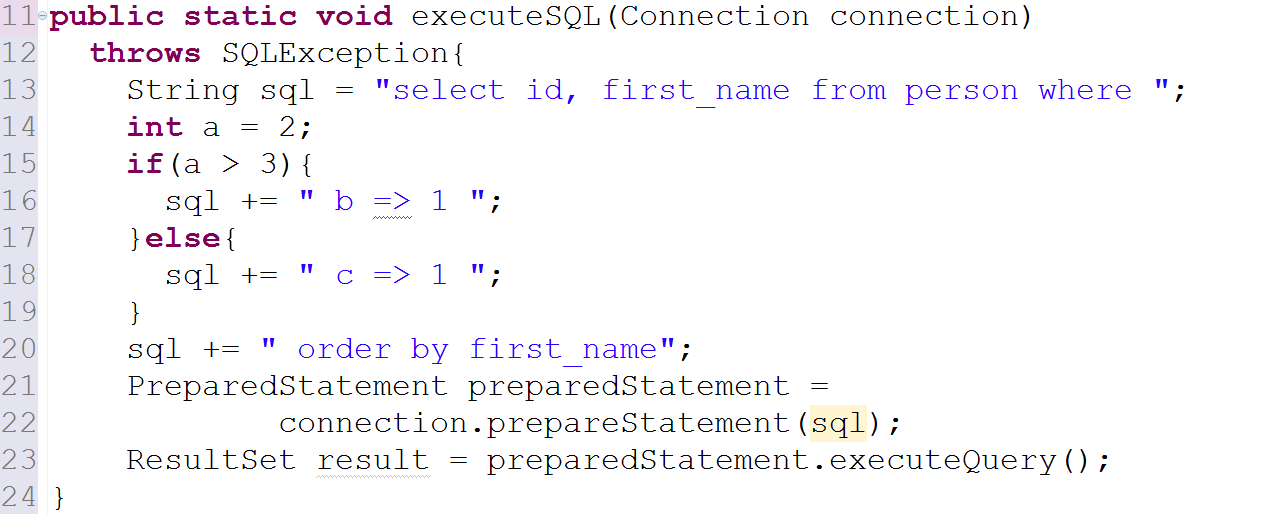
\includegraphics[scale=0.30]{Figures/Alvor.png}
    \end{center}
    \caption{Eclipse's text editor window with Alvor plugin}
    \label{alvor_pic}
\end{figure}

\subsection{IntelliLang}

IntelliLang\footnote{IntelliLang is a plugin offering a number of features related to the processing of embedded languages. Site: \url{https://www.jetbrains.com/idea/help/intellilang.html}} is a plugin for  IntelliJ IDEA\footnote{IntelliJ IDEA is an IDE for JVM-based development. Site: \url{http://www.jetbrains.com/idea/}} IDE that extends its functionality in the field of string-embedded languages support. Plugin can highlight embedded code, perform code completion and for some languages (JavaScript, XML) detect errors. IntelliLang does not perform strings with embedded code search: user should manually specify the strings to be analyzed. This makes it inconvenient to use the plugin for some tasks especially for reengineering. IntelliJ IDEA's text editor window is illustrated in Figure~\ref{IntelliLang_pic}. The method getHtml is marked by \verb|@Language("HTML")| attribute which means this method returns the string containing html code as a result. Despite the closing tag \verb|</body>| is missing in the 12 line, IntelliLang does not report the error as the plugin is not able to perform error checking for html language.

\begin{figure}[h!]
    \begin{center}
        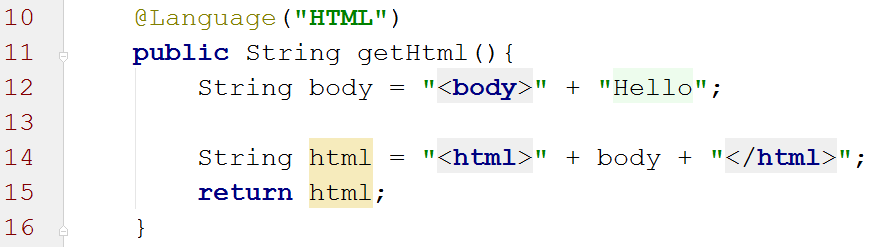
\includegraphics[scale=0.35]{Figures/IntelliLang.PNG}
    \end{center}
    \caption{IntelliJ IDEA's text editor window with IntelliLang plugin}
    \label{IntelliLang_pic}
\end{figure} 

\subsection{PhpStorm}

PhpStorm\footnote{IDE for PHP programming language. Site: \url{http://www.jetbrains.com/phpstorm/}} is an IDE for web-applications creating in PHP. PHP programs often contain embedded code in HTML, CSS, JavaScript, and SQL, and PhpStorm performs highlighting and code completion for it. However PhpStorm is not able to handle dynamically generated strings. Such an example can be seen in Figure~\ref{PHPStorm_pic}. The variable \verb|$string| contains html code, but it is not highlighted as its value is dynamically constructed. Moreover, PhpStorm does not report errors: even though the IDE highlighted the SQL code in the line 11, it did not indicate the error the query contains.

\begin{figure}[h!]
    \begin{center}
        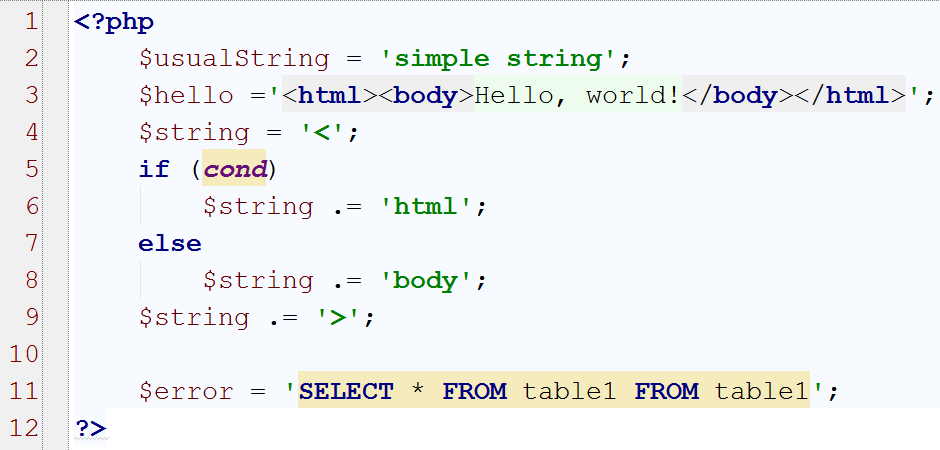
\includegraphics[scale=0.30]{Figures/PHPStorm.png}
    \end{center}
    \caption{PHPStorm's text editor window}
    \label{PHPStorm_pic}
\end{figure} 

\subsection{Varis}

Varis~\cite{Varis:ref} is a plugin for Eclipse that provides support of HTML, CSS, and JavaScript code embedded into PHP. The functionality includes code highlighting, completion, "jump to declaration", call graphs building for embedded JavaScript. Figure~\ref{varis_pic} illustrates code highlighting and completion functions. 

\begin{figure}[h!]
    \begin{center}
        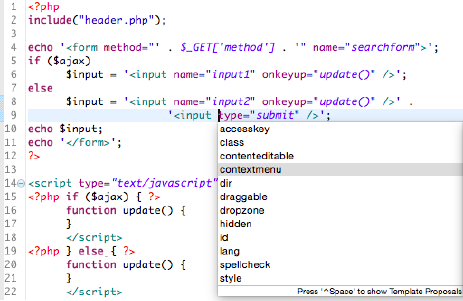
\includegraphics[scale=0.60]{Figures/Varis.PNG}
    \end{center}
    \caption{Eclipse's text editor window with Varis plugin}
    \label{varis_pic}
\end{figure} 

In conclusion one should note that along with specific drawbacks described tools either have limited functionality (JSA, PHPSA) which is difficult to extend, or support limited number of embedded languages (Alvor, PhpStorm and Varis). Furthermore, almost all the tools work with one specific host language.